\documentclass{book}

%%Packages:

\usepackage[utf8]{inputenc}
\usepackage[UKenglish]{babel}
\usepackage{graphicx}
\usepackage{cite}
\usepackage[hidelinks]{hyperref}
\usepackage{listings}
\usepackage{latexsym}
\usepackage{amsmath,amsthm,amssymb}
\usepackage{proof}
\usepackage{stmaryrd}
\usepackage{epstopdf}
\usepackage{pgf}
\usepackage{tikz}
\usepackage{algorithm}
\usepackage[noend]{algpseudocode}
\usetikzlibrary{automata,arrows,decorations.pathreplacing}
\usetikzlibrary{positioning}

%Symbols:

\let\emptyset\varnothing

%%Notation:

%%vectors
\renewcommand{\vec}[1]{\boldsymbol{#1}}
%%sets
\newcommand{\set}[1]{\mathcal{#1}}
%%matrixes
\newcommand{\mat}[1]{#1}
%%norm
\newcommand{\norm}[1]{\left\Vert #1 \right\Vert}

%%Envirorments:

% \newtheoremstyle{definition}{}{}{\itshape}{}{\bfseries}{.}{.5em}{\thmnote{#3's }#1}
\theoremstyle{definition}
\newtheorem{defn}{Definition}
\theoremstyle{definition}
\newtheorem{remark}{Remark}

%Paths:

\graphicspath{ {./images/} }

\title{On recurrent neural networks}
\author{Giulio Galvan}

%%%%%%%%%%%%%%%%%%%%%%%%%%%%%%%%%%%%

\begin{document}
\maketitle
\tableofcontents
\chapter{Artificial neural networks}
\section{A family of models}
 
An artificial neural network is a network of connected units called neurons or perceptrons, as can be seen in figure \ref{fully_connected}; the link which connects neurons $i$ and $j$, is associated with a weight $w_{ji}$. Perceptrons share the same
structure for all models, what really distinguish a particular model in the family of artificial neural networks is how the perceptron units are arranged and connected together, for example whether there are cycles
or not, and how data inputs are \textit{fed} to the network. 


\tikzstyle{nn_style}=[->,shorten >=1pt,auto,node distance=1.5cm,
  thick,
  neuron/.style={circle,fill=white!50,node distance=2cm,draw,minimum size=0.7cm,font=\sffamily\normalsize},
  missing/.style={circle,font=\sffamily\Large,node distance=0.95cm},
  label/.style={node distance=1.2cm,rectangle,fill=white!50,draw=none,minimum size=0.7cm,font=\sffamily\normalsize},
  layer/.style={rectangle,fill=white!50,draw,minimum width=1.5cm,font=\sffamily\Large},
  loopStyle/.style={in=120,out=60, distance=2.5cm},
  weight/.style = {above,sloped,pos=0.3},
  thin_edge/.style={line width=0.5pt}]
\begin{figure}[h]
 \centering
\begin{tikzpicture}[nn_style]
   
   \def\layersep{1.5cm}
  
    % Draw the input layer nodes
    \foreach \name / \y in {1,...,4}
    % This is the same as writing \foreach \name / \y in {1/1,2/2,3/3,4/4}
        {\node[neuron] (I-\name) at (\y *1.5,0) {};
        \node[label] (I-\name-label) [below of=I-\name] {$x_\y$};
        }
        
    \foreach \name / \y in {1,...,4}
        \path[->,thin_edge] (I-\name-label)edge[] (I-\name); 

    % Draw the hidden layer nodes
    \foreach \name / \y in {1,...,5}
        \path[yshift=0.5cm,thin_edge]
            node[neuron] (H-\name) at (\y *1.5  -0.9, \layersep) {};

    % Draw the output layer nodes
    \foreach \name / \y in {1,...,3}{
        \path[yshift=0.5cm,thin_edge]
            node[neuron] (O-\name) at (\y *1.5 + 0.6, \layersep*2) {};
         \node[label] (O-\name-label) [above of=O-\name] {$y_\y$};

            }
    \foreach \name / \y in {1,...,3}
        \path[->,thin_edge] (O-\name)edge[] (O-\name-label); 

    % Connect every node in the input layer with every node in the
    % hidden layer.
    \foreach \source in {1,...,4}
        \foreach \dest in {1,...,5}
            \path[thin_edge] (I-\source) edge (H-\dest);
            
    % Connect every node in the hidden layer with every node in the
    % output layer.
    \foreach \source in {1,...,5}
        \foreach \dest in {1,...,3}
            \path[thin_edge] (H-\source) edge (O-\dest);
            

\end{tikzpicture}
\caption{Artificial neural network example}
\label{fully_connected}
\end{figure}


As you can see in figure \ref{neuron_model} each neuron is \textit{fed} with a set inputs which are the weighted outputs of other neurons and/or other external inputs.
Formally the output of a perceptron $\phi_j$
is defined as:
 
\begin{align}
&\phi_j \defeq \sigma(a_j)\label{def_perceptron_1}\\
&a_j \defeq \sum_l w_{jl}\phi_l +b_j \label{def_perceptron_2}
\end{align}

where $w_{jl}$ is the weight of the connection between neuron $l$ and neuron $j$, $\sigma(\cdot)$ is a non linear function and $b_j \in \mathbb{R}$ is a bias term.
It's worth noticing that in this formulation the input $\phi_l$ can be the outputs of other neurons or provided external inputs.


\tikzstyle{nn_style}=[->,shorten >=1pt,auto,node distance=1.5cm,
  thick,
  neuron/.style={circle,fill=white!50,node distance=1cm,draw,minimum size=0.7cm,font=\sffamily\normalsize},
  missing/.style={circle,font=\sffamily\Large,node distance=0.95cm},
  label/.style={node distance=1.2cm,rectangle,fill=white!50,draw=none,minimum size=0.7cm,font=\sffamily\normalsize},
  layer/.style={rectangle,fill=white!50,draw,minimum width=1.5cm,font=\sffamily\Large},
  loopStyle/.style={in=120,out=60, distance=2.5cm},
  weight/.style = {above,sloped,pos=0.3},]
\begin{figure}[h]
 \centering
\begin{tikzpicture}[nn_style]

  \node[neuron]    (x0)       {};
  \node[neuron]    (x1)[below of=x0]   {};
  \node[neuron]    (x2)[below of=x1]   {};
  \node[missing]   (x3)[below of=x2]   {$\vdots$};
  \node[neuron]    (xn)[below of=x3]   {};
  
  
  \node[label]    (u0)[left of=x0]   {$\phi_0$};
  \node[label]    (u1)[left of=x1]   {$\phi_1$};
  \node[label]    (u2)[left of=x2]   {$\phi_2$};
  \node[label]    (un)[left of=xn]   {$\phi_n$};
  
  
  \node[layer] (hl)[ right of=x2,node distance=3.5cm] {$\Sigma$};
  \node[neuron](bias)[above of=hl,node distance=2cm]{$1$};
  \node[layer] (ol)[right of=hl,node distance=2.5cm] {$\sigma$};
  
  \node[label]  (phi)[right of=ol,node distance=2cm] {$\phi_j$};
   
  
  \path[->] (x0) edge [] node[weight]{$w_{0j}$}   (hl)
	    (x1) edge [] node[weight]{$w_{1j}$}   (hl)
	    (x2) edge [] node[weight]{$w_{2j}$}   (hl)
	    (xn) edge [] node[weight]{$w_{nj}$}   (hl)
 	    (bias) edge[]  node[]{$b_{j}$}(hl)
	    (u0) edge []   (x0)
	    (u1) edge []   (x1)
	    (u2) edge []   (x2)
	    (un) edge []   (xn)
	    (hl) edge []   node[]{$a_{j}$}(ol)
	    (ol) edge []   (phi);

\end{tikzpicture}
\caption{Neuron model}
\label{neuron_model}
\end{figure}

So, given a set of inputs $\{x\}_i$ which are \textit{fed} to some of the units of the net which we call \textit{input units} the output of the network $\{y\}_i$ is given by the
some of units of the network, the 'upper' ones which we call \textit{output units}. All remaining units, i.e the ones which are neither input nor output units
are called \textit{hidden units} because their value is not \textit{observed} from the outside. The mapping from input to output is captured by equations \ref{def_perceptron_1} and 
\ref{def_perceptron_2}. 

\paragraph{The activation function}
The $\sigma$ function is called \textit{activation} function and should determine whether a perceptron unit is \textit{active} or not. When artificial neural networks where first conceived,
trying to mimic the brain structure, such function was a simple threshold function, trying to reproduce the behaviour of brain neurons: a neuron is \textit{active}, i.e it's output $\phi_j$ is $1$, if
the sum of input stimuli $\sum_l w_{jl}\phi_l +b_j$ is greater than a given threshold $\tau$.

\begin{equation}
  \sigma_{\tau}(x)=\begin{cases}
    1 & \text{if $x>\tau$}.\\
    0 & \text{otherwise}.
  \end{cases}
\end{equation}
Such function, however, is problematic when we are to compute gradients because it's not continuous, so one of the following function is usually chosen:

\begin{equation}
 sigmoid(x)=\frac{1}{1+e^{-x}}
\end{equation}
\begin{equation}
 tanh(x)=\frac{e^x-e^{-x}}{e^x+e^{-x}}
\end{equation}
These functions behave similarly to the threshold function, but, because of their \textit{smoothness}, present no problems in computing gradients.
Another function which is becoming a very popular choice is the \textit{rectified linear unit}:
\begin{equation}
  ReLU(x)=\begin{cases}
    x & \text{if $x>0$}.\\
    0 & \text{otherwise}.
  \end{cases}
\end{equation}
ReLU activation function is rather different from previous activation functions, some of these difference, in particular with respect to gradients will be analysed in later sections.

It's worth noticing that the activation function it's the only component which make artificial neuron networks a non linear model. Were we to choose a \textit{linear} function as activation function we will
end up with a simple linear model since the outputs of the network would be ultimately composed only of sums of products.

\paragraph{The bias term}
Let's consider the old threshold function $\sigma_{\tau}$, and ask ourselves what the bias term is for, what does changing this term bring about.
Suppose neuron $j$ has no bias term, the neuron value would be $a_j = \sum_l w_{jl}\phi_l$; if $a_j>\tau$ that neuron is active otherwise it is not. Now, let's add the bias term to $a_j$;
we obtain that neuron $j$ is active if $a_j>\tau-b_j$. So the effect of the bias term is to change the activation threshold of a given neuron. Using bias terms in a neural network architecture gives us
the ability to change the activation threshold for each neuron; that's particularly important considering that we can learn such bias terms.
We can do these same considerations in an analogous way for all the other activation functions.
\paragraph{Layered view of the net}
It's often useful to think of a neural network as series of layers, one on top of each other, as depicted in figure \ref{layered_nnet}. The first layer is called the input layer and its units are \textit{fed}
with external inputs, the upper layers are called \textit{hidden layers} because theirs outputs are not observed from outside except the last one which is called \textit{output layer} because it's output 
is the output of the net.

When we describe a network in this way is also useful to adopt a different notation: we describe the weights of the net with a set of matrices $\mat{W^k}$ one for each layer, and neurons are no more
globally indexed, instead with refer to a neuron with a relative index with respect to the layer; this allows to write easier equations in matrix notation
\footnote{In the rest of the book we will refer to the latter notation as \textsl{layer notation} and to the previous one as \textsl{global notation}}.
In this notation $\mat{W^k}_{ij}$ is the weight of the link connecting neuron $j$ of layer $k-1$ to neuron $i$ of level $k$


\tikzstyle{rnn_style}=[->,shorten >=1pt,auto,node distance=1.5cm,
  thick,
  neuron/.style={circle,fill=white!50,draw,node distance = 1cm, minimum size=0.7cm,font=\sffamily\Large\bfseries},
  missing/.style={rectangle,fill=white!50,node distance =1cm,draw=none,minimum size=0.7cm,font=\sffamily\Huge\bfseries},
  label/.style={node distance=1.2cm,rectangle,fill=white!50,draw=none,minimum size=0.7cm,font=\sffamily\normalsize},
  layer/.style={rectangle,fill=white!50,draw,minimum width=4cm,font=\sffamily\normalsize},
  loopStyle/.style={in=120,out=60, distance=2.5cm},]
\begin{figure}
 \centering
\begin{tikzpicture}[rnn_style]

  \node[neuron]    (x0)       {};
  \node[neuron]    (x1)[right of=x0]   {};
  \node[neuron]    (x2)[right of=x1]   {};
  \node[missing]   (x3)[right of=x2]   { $\hdots$};
  \node[neuron]    (xn)[right of=x3]   {};
  
  \node[label]    (u0)[below of=x0]   {$x_0$};
  \node[label]    (u1)[below of=x1]   {$x_1$};
  \node[label]    (u2)[below of=x2]   {$x_2$};
  \node[label]    (un)[below of=xn]   {$x_p$};
  
  

    
  \node[layer] (hl)[above of=x2,node distance=1.5cm] {First hidden layer};
  \node[missing] (hls)[above of=hl,node distance=1.2cm]{$\hdots$};
  \node[layer] (ol)[above of=hls,node distance=1.2cm] {Last hidden layer};
  
  \draw[decorate,decoration={brace,raise=6pt,amplitude=8pt}, thick,-]
   (ol.north east)--(hl.south east);



  
  \node[neuron] (o1) at (0,5.5) {};
  \node[neuron] (o2)[right of=o1] {};
  \node[neuron] (o3)[right of=o2] {};
  \node[missing](o4)[right of=o3] {$\hdots$};
  \node[neuron] (on)[right of=o4] {};
  
  
  \node[label]    (y0)[above of=o1]   {$y_0$};
  \node[label]    (y1)[above of=o2]   {$y_1$};
  \node[label]    (y2)[above of=o3]   {$y_2$};
  \node[label]    (yn)[above of=on]   {$y_q$};
  
     
  \node[label]    (hls_label)[right of=hls,node distance=3.7cm]   {hidden layers};
  \node[label]    (input_label)[right of=xn,node distance=1.6cm]   {input layer};
  \node[label]    (output_label)[right of=on,node distance=1.6cm]   {output layer};
  
  
  \path[->] (x0) edge [] node[]{}   (hl)
	    (x2) edge []   (hl)
	    (x1) edge []   (hl)
	    (xn) edge []   (hl)
	    (u0) edge []   (x0)
	    (u1) edge []   (x1)
	    (u2) edge []   (x2)
	    (un) edge []   (xn)
	    (ol) edge []   (o1)
	    (ol) edge []   (o2)
	    (ol) edge []   (o3)
	    (ol) edge []   (on)
	    (o1) edge []   (y0)
	    (o2) edge []   (y1)
	    (o3) edge []   (y2)
	    (on) edge []   (yn)
	    (hl) edge []  node[]{} (hls)
	    (hls) edge []  node[]{} (ol);


\end{tikzpicture}
\caption{Layered structure of an artificial neural network}
\label{layered_nnet}
\end{figure}
\section{Feed foward neural networks}

A feed forward neural network is an artificial neural network in which there are no cycles, that is to say each layer output is \textit{fed} to the 
next one and connections to earlier layers are not possible. 


\begin{defn}[Feed forward neural network]
\label{def_ffnn}
A feed forward neural network is tuple:
$$\net{FFNN}\defeq<\vec{p},\set{W},\set{B},\sigma(\cdot),F(\cdot)>$$
\begin{itemize}
 \item $\vec{p} \in \mathbb{N}^U$ is the vector whose elements $p(k)$ are the number of neurons of layer $k$; $U$ is the number of layers
 \item $\set{W} \defeq \{W^k_{p(k+1) \times p(k)}, k=1,...,U-1 \}$ is the set of weight matrices of each layer
 \item $\set{B} \defeq \{\vec{b}^k \in \mathbb{R}^{p(k)}, k=1,...,U \} $ is the set of bias vectors
 \item $\sigma(\cdot): \mathbb{R}\rightarrow \mathbb{R}$ is the activation function
 \item $F(\cdot): \mathbb{R}^{p(U)}\rightarrow \mathbb{R}^{p(U)}$ is the output function
\end{itemize}
\end{defn}

\begin{remark}{}
Given a $\net{FFNN}$:
\begin{itemize}
 \item The number of output units is $p(U)$
 \item The number of input units is $p(1)$
 \item The total number of weights is $\mathcal{N}(\set{W}) \defeq \sum_{k=1}^U p(k+1)p(k)$
 \item The total number of biases is $\mathcal{N}(\set{B}) \defeq \sum_{k=1}^{U} p(k)$
\end{itemize}
\end{remark}

\begin{defn}[Output of a $\net{FFNN}$]
Given a $\net{FFNN}$ and an input vector $\vec{x} \in \mathbb{R}^{p(1)}$ the output of the net $\vec{y} \in \mathbb{R}^{p(U)}$  is defined by the following:

\begin{align}
&\vec{y}=F(\vec{a}^{U}) &\\
&\vec{\phi}^{i} \defeq \sigma(\vec{a}_{i}), & i=1,...,U\\
&\vec{a}^{i} \defeq W^{i-1} \cdot \vec{\phi}^{i-1} +\vec{b}^i  & i=1,...,U\\
&\vec{\phi}^{1} \defeq \vec{x} &
\end{align}
\end{defn}

\subsection{Learning with FFNNs}
A widespread application of neural networks is that of machine learning. In the following we will model an optimisation problem which rely on $\net{FFNNs}$.
To model an optimisation problem we first need to define a data-set $D$ as 
\begin{equation}
D\defeq\{\overline{\vec{x}}^{(i)} \in \mathbb{R}^p, \overline{\vec{y}}^{(i)} \in \mathbb{R}^q,  i=1,...,N\}
\end{equation}
Then we need a loss function $L_D:\mathbb{R}^{\mathcal{N}(\set{W})+\mathcal{N}(\set{B})} \rightarrow \mathbb{R}_{\geq 0}$ over $D$ defined as
\begin{equation}
L_D(\set{W},\set{B})\defeq\frac{1}{N}\sum_{i=1}^N L(\overline{\vec{x}}^{(i)},\vec{y}^{(i)}) 
\end{equation}
$L(\vec{x},\vec{y}):\mathbb{R}^{p(U)} \rightarrow \mathbb{R}$ is an arbitrary loss function computed on the $i^{th}$ example. Note that $\vec{y}$ is the output of the
networks, so it depends on $(\set{W},\set{B})$


The problem is then to find a $\net{FFNN}$ which minimise $L_D$. As we have seen feed forward neural networks allow for large customisation: the only variables in the optimisation problem are the weights
and the biases, the other
parameters are said \textit{hyper-parameters} and are determined \textit{a priori}. Usually the output function is chosen depending on the output, for instance for multi-way classification
is generally used the \textit{softmax} function, for regression a simple identity function.
For what concerns the number of layers and the number of units per layers they are chosen relying on experience or performing some kind of hyper-parameter tuning, which usually consists on training nets
with some different configurations of such parameters and choosing the 'best one'.

Once we have selected the values for all hyper-parameters the optimisation problem becomes:

\begin{equation}
\underset{\set{W},\set{B}}{\text{min  }} L_D(\set{W},\set{B}) \\
\end{equation}


\subsection{Gradient}
Consider a $\net{FFNN}=\langle\vec{p},\set{W},\set{B},\sigma(\cdot),F(\cdot)\rangle$, let $L:\mathbb{R}^{p(U)} \times \mathbb{R}^{p(U)} \rightarrow \mathbb{R}$ a loss function and 
$g(\cdot):\mathbb{R}^{\mathcal{N}(\set{W})+\mathcal{N}(\set{B})} \rightarrow \mathbb{R}$ be the function defined by
\begin{equation}
g(\set{W},\set{B}) \defeq L(F(a^U( \overline{\vec{y}}^{(i)} )),\vec{y}^{(i)}(\set{W},\set{B}) ).
\label{loss_over_y_i}
\end{equation}
Equation (\ref{loss_over_y_i}), tough it seems rather scary, express a very simple thing: we consider a single input example 
$\overline{\vec{x}}^{(i)}$, we run it through the network and we confront it's output $F(a^U( \overline{\vec{x}}^{(i)}) $ with it's label
$\overline{\vec{y}}^{(i)}$ using the loss function $L$; the function $g(\set{W},\set{B})$ it's simply the loss function computed on the $i^{th}$ example
which of course depends only on the weights and biases of network since the training examples are fixed within the dataset. In the following we will derive an expression for gradient with respect to a weight matrix $\mat{W}^{i}$ and a bias vector $\vec{b}^i$. Before reading further consider taking a look at the notation appendix.
\begin{align}
\label{eq:ffnnGradientJacobian}
\frac{\partial g}{\partial \mat{W}^i} &= \nabla L^T \cdot J(F) \cdot  \frac{\partial \vec{y}}{\partial \vec{a}^U} \cdot \frac{\partial \vec{a}^U}{\partial \mat{W}^i}\\
&= \frac{\partial g}{\partial \vec{a}^U} \cdot \frac{\partial \vec{a}^U}{\partial \mat{W^i}}.
\end{align}

To help clarify the notation we provide just for equation \ref{eq:ffnnGradientJacobian} the dimensions of the matrices involved in the product:
$$[1\times p(i+1)\cdot p(i)] = [p(U)\times 1] \cdot [p(U)\times p(U)] \cdot [p(U)\times p(i+1)\cdot p(i)].$$ 

We can easily compute the gradient of $L$, $\nabla L$, and the jacobian of $F$, $J(F)$, once we define $F(\cdot)$ and $L(\cdot)$. Note that the weights are not involved in such computation.
Let us derive an expression for $\frac{\partial \vec{a}^U}{\partial \mat{W}^i}$.
We will start deriving such derivative using the global notation. Consider a single output unit $u$ and a weight $w_{lj}$ linking neuron $j$ to neuron $l$.


\begin{align}
\frac{\partial a_u}{\partial w_{lj}} &= \frac{\partial a_u}{\partial a_l} \cdot \frac{\partial a_l}{\partial w_{lj}}\\
&=\delta_{ul} \cdot h_j,
\end{align}

where we put $$\delta_{ul} \defeq \frac{\partial a_u}{\partial a_l}.$$

Let $P(l)$ be the set of parents of neuron $l$, formally:
\begin{equation} 
P(l) = \{ k: \exists \text{ a link between $l$ and $k$ with weight } w_{lk} \}.
\end{equation}
We can compute $\delta_{ul}$ simply applying the chain rule, if we write it down in bottom-up style, as can be seen in Figure \ref{deriv_arcs}, we obtain:
\begin{equation}
\delta_{ul} = \sum_{k\in P(l)} \delta_{uk} \cdot \sigma'(a_k)\cdot w_{kl}.
\end{equation}

\tikzstyle{rnn_style}=[->,shorten >=1pt,auto,node distance=1.5cm,
  thick,
  neuron/.style={circle,fill=white!50,draw,minimum size=0.7cm,font=\sffamily\normalsize},
  missing/.style={circle,fill=white!50,draw=none,minimum size=0.7cm,font=\sffamily\Huge\bfseries},
  label/.style={node distance=1.2cm,rectangle,fill=white!50,draw=none,minimum size=0.7cm,font=\sffamily\normalsize},
  thick/.style={line width=1.2pt},
  thin_edge/.style={line width=0.5pt}
  ]
\begin{figure}
 \centering
\begin{tikzpicture}[rnn_style]

  \node[neuron]    (u)       {$u$};
  
  \node[neuron,thick]    (x1)[left of=u, below of=u]   {};
  \node[neuron,thick]    (x2)[right of=x1]   {};
  \node[neuron,thick]    (x3)[right of=x2]   {};
  
  \node[neuron]    (y1)[below of=x1]   {$l$};
  \node[neuron]    (y2)[right of=y1]   {};
  \node[neuron]    (y3)[right of=y2]   {};
  
  \node[neuron]    (z1)[below of=y1]   {};
  \node[neuron]    (z2)[right of=z1]   {};
  \node[neuron]    (z3)[right of=z2]   {};
  
%   \node[label]      (lu)[left of=u] {$u$};
%   \node[label]      (ll)[left of=z1] {$l$};
  
  
  \path[->] (x1) edge [thick] node[]{}   (u)
	    (x2) edge [thick]   (u)
	    (x3) edge [thick]   (u)
	    (y1) edge [thick]   (x1)
	    (y1) edge [thick]   (x2)
	    (y1) edge [thick]   (x3)
	    (y1) edge [thin_edge]   (x2)
	    (y2) edge [thin_edge]   (x3)
	    (y3) edge [thin_edge]   (x1)
	    (y1) edge [thin_edge]   (x3)
	    (y2) edge [thin_edge]   (x2)
	    (y3) edge [thin_edge]   (x1)
	  
	    (z1) edge [thin_edge]   (y1)
	    (z1) edge [thin_edge]   (y2)
	    (z1) edge [thin_edge]   (y3)
	    (z1) edge [thin_edge]   (y2)
	    (z2) edge [thin_edge]   (y3)
	    (z3) edge [thin_edge]   (y1)
	    (z1) edge [thin_edge]   (y3)
	    (z2) edge [thin_edge]   (y2)
	    (z3) edge [thin_edge]   (y1);


\end{tikzpicture}
\caption{Nodes and edges involved in $\frac{\partial a_u }{\partial a_l}$.}
\label{deriv_arcs}
\end{figure}

The derivatives with respect to biases are computed in the same way:

\begin{align}
\frac{\partial a_u}{\partial b_{l}} &= \frac{\partial a_u}{\partial a_l} \cdot \frac{\partial a_l}{\partial b_{l}}\\
&=\delta_{ul} \cdot 1.
\end{align}



In layered notation we can rewrite the previous equations as:
\begin{equation}
 \frac{\partial a^U}{\partial \mat{W}^i} = \frac{\partial a^U}{\partial a^{i+1}} \cdot \frac{\partial^{+} a^{i+1}}{\partial \mat{W}^i},
\end{equation}


\begin{equation}
\frac{\partial^{+} a^{i+1}}{\partial \mat{W}_j^i} =
 \begin{bmatrix}
   h_j^{i}    & 0                & \cdots      & \cdots       & 0  \\
   0               & h_j^{i}     & \cdots      & \cdots       & 0  \\
   \vdots          & \vdots           & \ddots      & \vdots       &\vdots\\
   0               & \cdots           & \cdots      & \cdots       & h^{i}_{j}
\end{bmatrix},
\end{equation}

\begin{equation}
\frac{\partial a^U}{\partial a^{i}} \defeq \Delta^{i} = 
\begin{cases}
      \Delta^{i+1} \cdot diag(\sigma'(\vec{a}^{i+1})) \cdot W^{i}  & \text{if } i<U,\\
      Id & \text{if } i==U,\\
    0 & \text{otherwise},
\end{cases}
\label{fnn_delta}
\end{equation}
where
\begin{equation}
diag(\sigma'(\vec{a}^{i})) =
 \begin{bmatrix}
   \sigma'(a^{i}_1)    & 0                & \cdots      & \cdots       & 0  \\
   0                     & \sigma'(a^{i}_2)     & \cdots      & \cdots       & 0  \\
   \vdots                & \vdots           & \ddots      & \vdots       &\vdots\\
   0                     & \cdots           & \cdots      & \cdots       &\sigma'(a^{i}_{p(i)})
\end{bmatrix}.
\end{equation}

The derivatives w.r.t the biases are instead:
\begin{align}
\frac{\partial a^U}{\partial b^i} &= \frac{\partial a^U}{\partial a^i} \cdot \frac{\partial a^i}{\partial b^i}\\
&= \Delta^{i} \cdot Id.
\end{align}


\paragraph{Backpropagation}

Previous equations are the core of the famous \textit{back-propagation} algorithm which was first introduced by Rumelhart et al.\cite{Rumelhart86}.
The algorithm consists in two \textit{passes}, a \textit{forward pass} and a \textit{backward pass} which give the name to the algorithm.
The \textit{forward pass} start from the first layer, compute the hidden units values and the proceed to upper layers using the value of the hidden units 
$\vec{a^i}$ of previous layers which have already been computed. The \textit{backward pass} instead, start from the topmost layer and computes $\Delta^{i}$
which can be computed, as we can see from equation \ref{fnn_delta} , once it is known $\Delta^{i+1}$, which has been computed in the previous step, and $\vec{a^i}$ which
has been computed in the \textit{forward pass}.

\textit{Backpropagation} algorithm has time complexity $\mathcal{O}(\mathcal{N}(\set{W}))$.




\section{Recurrent neural networks}
Recurrent neural networks differ from feed forward neural networks because of the presence of recurrent connections: at least one perceptron output at a given layer $i$ is \textit{fed} to another perceptron
at a level $j<i$, as can be seen in Figure \ref{rnn_model}. 
This is a key difference, as we will see in later sections, because it introduces \textit{memory} in the network, changing, somehow, the expressiveness
of the model.


\tikzstyle{rnn_style}=[->,shorten >=1pt,auto,node distance=1.5cm,
  thick,
  neuron/.style={circle,fill=white!50,node distance =1.2cm,draw,minimum size=0.7cm,font=\sffamily\Large\bfseries},
  missing/.style={rectangle,node distance =1.2cm,fill=white!50,draw=none,minimum size=0.7cm,font=\sffamily\Huge\bfseries},
  label/.style={node distance=1.2cm,rectangle,fill=white!50,draw=none,minimum size=0.7cm,font=\sffamily\normalsize},
  layer/.style={rectangle,fill=white!50,draw,minimum width=4cm,font=\sffamily\normalsize},
  loopStyle/.style={in=120,out=60, distance=2.5cm},]
\begin{figure}[!h]
 \centering
\begin{tikzpicture}[rnn_style]

  \node[neuron]    (x0)       {};
  \node[neuron]    (x1)[right of=x0]   {};
  \node[neuron]    (x2)[right of=x1]   {};
  \node[missing]   (x3)[right of=x2]   { $\hdots$};
  \node[neuron]    (xn)[right of=x3]   {};
  
  \node[label]    (u0)[below of=x0]   {$u_0[t]$};
  \node[label]    (u1)[below of=x1]   {$u_1[t]$};
  \node[label]    (u2)[below of=x2]   {$u_2[t]$};
  \node[label]    (un)[below of=xn]   {$u_n[t]$};
  
  
  \node[layer] (hl)[above of=x2,node distance=2cm] {Hidden layer};
  \node[neuron](b) [right of=hl,node distance=3cm] {};
  \node[label] (b_l) [right of=b] {bias=1};
  \node[layer] (ol)[above of=hl,node distance=2cm] {Output layer};
  
  \node[neuron] (o1) at (0,5.5) {};
  \node[neuron] (o2)[right of=o1] {};
  \node[neuron] (o3)[right of=o2] {};
  \node[missing](o4)[right of=o3] {$\hdots$};
  \node[neuron] (on)[right of=o4] {};
  
  
  \node[label]    (y0)[above of=o1]   {$y_0[t]$};
  \node[label]    (y1)[above of=o2]   {$y_1[t]$};
  \node[label]    (y2)[above of=o3]   {$y_2[t]$};
  \node[label]    (yn)[above of=on]   {$y_n[t]$};
  
  
  \path[->] (x0) edge [] node[]{$W_{in}$}   (hl)
	    (x1) edge []   (hl)
	    (x2) edge []   (hl)
	    (xn) edge []   (hl)
	    (u0) edge []   (x0)
	    (u1) edge []   (x1)
	    (u2) edge []   (x2)
	    (un) edge []   (xn)
	    (ol) edge []   (o1)
	    (ol) edge []   (o2)
	    (ol) edge []   (o3)
	    (ol) edge []   (on)
	    (o1) edge []   (y0)
	    (o2) edge []   (y1)
	    (o3) edge []   (y2)
	    (on) edge []   (yn)
	    (hl) edge []  node[]{$W_{out}$} (ol)
	    (b)  edge [bend left,dotted,in= 160]  node[]{$b_{rec}$} (hl)
	    (b)  edge [bend left,dotted,anchor=west, in= -160]  node[]{$b_{out}$} (ol)
	    (hl) edge [loop ,in=-160,out=160, distance=3cm,anchor=east ]      node [align=center]  {$W_{rec} $} (hl);

\end{tikzpicture}
\caption{$\net{RNN}$ model.}
\label{rnn_model}
\end{figure}


This difference in topology reflects also on the network's input and output domain: where, in feed forward neural networks, inputs and outputs were real valued vectors, recurrent neural networks deal with
sequences of vectors; in other words time is also considered. One may argue that, taking time (and sequences) into consideration, is some sort of a limitation, because it restricts our model to deal only
with temporal inputs; however that's not the case, in fact we can apply RNNs to non temporal data by considering space as the temporal dimension, for example imagine feeding the network with the pixels of an image one column at a time; or we can feed the network with the same input for all time steps or simply
providing no input at all after the first step.

\begin{defn}[Recurrent neural network]
\label{def_rnn}
A recurrent  neural network is tuple
$$\net{RNN}\defeq\langle \set{W},\set{B} ,\sigma(\cdot),F(\cdot)\rangle$$
\begin{itemize}
 \item $\set{W} \defeq \{\mat{W}^{in},\mat{W^{rec},\mat{W^{out}}}\}$ where
 \begin{itemize}
  \item $W^{in}$ is the $r\times p$ input weight matrix
  \item $W^{rec}$ is the $r\times r$ recurrent weight matrix
  \item $W^{out}$ is the $o \times r$ output weight matrix
 \end{itemize}
 \item $\set{B} \defeq \{\vec{b^{rec},\vec{b^{out}}}\}$ where
 \begin{itemize}
   \item $\vec{b}^{rec} \in \mathbb{R}^{r}$ is the bias vector for the recurrent layer
   \item $\vec{b}^{out} \in \mathbb{R}^{o}$ is the bias vector for the output layer
 \end{itemize}
 \item $\sigma(\cdot): \mathbb{R}\rightarrow \mathbb{R}$ is the activation function
 \item $F(\cdot): \mathbb{R}^{o}\rightarrow \mathbb{R}^{o}$ is the output function.
\end{itemize}
\end{defn}

\begin{remark}{}
Given a $\net{RNN}$
\begin{itemize}
 \item the total number of weights is given by $\mathcal{N}(W) \defeq rp+r^2+ro$
 \item the number of biases by $\mathcal{N}(b) \defeq r+o $
 \item $p$ is the size of input vectors
 \item$r$ is the number of hidden units
 \item $o$ is the size of output vectors. 
\end{itemize}
\end{remark}

\begin{defn}[Output of a $\net{RNN}$]
\label{def_rnn_output}
Given a $\net{RNN}$ and an input sequence $\{\vec{x}\}_{t=1,...,T}$, with $ \vec{x}_t \in \mathbb{R}^p$, the output sequence of the net $\{\vec{y}\}_{t=1,...,T}$, with $\vec{y}_t \in \mathbb{R}^o$,  is defined by the following:
\begin{align}
&\vec{y}^t \defeq F(W^{out}\cdot\vec{a}^t + \vec{b}^{out})\\
&\vec{a}^t \defeq W^{rec}\cdot\vec{h}^{t-1}+W^{in}\cdot\vec{x}^t+\vec{b}^{rec}\\
&\vec{h}^t \defeq  \sigma(\vec{a}^t) \\
&\vec{h}^0 \defeq \overrightarrow{0}.
\end{align}
\end{defn}
As we can understand from definition \ref{def_rnn_output}, there is only one recurrent layer, whose weights are the same for each time step, so one could asks where does the deepness of the network come from.
The answer lies in the temporal unfolding of the network, in fact if we unfold the network step by step we obtain a structure similar to that of a feed forward neural network. As we can observe
in Figure \ref{rnn_unfolding}, the unfolding of the network through time consist of putting identical version of the same recurrent layer one on top of each other and linking the inputs of one layer to the
next one. The key difference from feed forward neural networks is, as we have already observed, that the weights in each layer are identical; another
important unlikeness is of course the presence of additional timed inputs for each unfolded layer.

\tikzstyle{rnn_style}=[->,shorten >=1pt,auto,node distance=1.5cm,
  thick,
  neuron/.style={circle,fill=white!50,draw,minimum size=0.7cm,font=\sffamily\Large\bfseries},
  missing/.style={circle,fill=white!50,draw=none,minimum size=0.7cm,font=\sffamily\Huge\bfseries},
  label/.style={node distance=1.2cm,rectangle,fill=white!50,draw=none,minimum size=0.7cm,font=\sffamily\normalsize},
  layer/.style={rectangle,fill=white!50,draw,minimum width=4cm,font=\sffamily\normalsize},
  loopStyle/.style={in=120,out=60, distance=2.5cm},]
\begin{figure}[h!]
 \centering
\begin{tikzpicture}[rnn_style]

  %t=0
  \node[layer] (hl1) {Hidden layer t=0};
  
  \node[neuron]    (x0)[below left=0.3cm and 1cm of hl1]       {};
  \node[label]    (u0)[left of=x0]   {$\vec{x}_1$};
  

  
  \node[neuron] (o0) [above right=0.3cm and 1cm of hl1] {};
  \node[label]    (y0)[right of=o0]   {$\vec{y}_1$};
  
  %t=1
  \node[layer] (hl2)[above of=hl1,node distance=2.5cm] {Hidden layer t=1};
  
  \node[neuron]    (x1)[below left=0.3cm and 1cm of hl2]      {};
  \node[label]    (u1)[left of=x1]   {$\vec{x}_2$};
  
    
  \node[neuron] (o1) [above right=0.3cm and 1cm of hl2] {};
  \node[label]    (y1)[right of=o1]   {$\vec{y}_2$};
  
  %dots
  \node[label,font=\sffamily\Huge\bfseries] (hld)[above of=hl2,node distance=2cm] {$\hdots$};
  
  %t=T
  \node[layer] (hlT)[above of=hld,node distance=2cm] {Hidden layer t=T};
  
  \node[neuron]    (xT)[below left=0.3cm and 1cm of hlT]      {};
  \node[label]    (uT)[left of=xT]   {$\vec{x}_T$};
  
    
  \node[neuron] (oT) [above right=0.3cm and 1cm of  hlT] {};
  \node[label]    (yT)[right of=oT]   {$\vec{y}_T$};
  
  
  %biases
  \node[neuron](b) [right of=y1,node distance=1.4cm] {};
  \node[label] (b_l) [above of=b,node distance=0.7cm] {bias=1};

  
  \path[->] (x0) edge [bend right] node[]{$W^{in}$}   (hl1)
	    (u0) edge []   (x0)
	    (o0) edge []   (y0)
	    (x1) edge [bend right] node[]{$W^{in}$} (hl2)
	    (u1) edge []   (x1)
    	    (o1) edge []   (y1)
	    (xT) edge [bend right] node[]{$W^{in}$} (hlT)
	    (uT) edge []   (xT)
    	    (oT) edge []   (yT)

	    
	    (hl1) edge [bend left]  node[]{$W^{out}$} (o0)
    	    (hl2) edge [bend left]  node[]{$W^{out}$} (o1)
    	    (hlT) edge [bend left]  node[]{$W^{out}$} (oT)

	    (b)  edge [bend left,dotted,in = 90]  node[]{$b^{out}$} (o0)
	    (b)  edge [bend left, dotted, in = 90,out=80]  node[]{$b^{rec}$} (hl1)
	    (b)  edge [bend left, dotted]  node[]{$b^{rec}$} (hl2)
	    (b)  edge [bend left,dotted]  node[]{$b^{out}$} (o1)
	    (b)  edge [bend left, dotted,in = 200]  node[]{$b^{rec}$} (hlT)
	    (b)  edge [bend left,dotted,in =200]  node[]{$b^{out}$} (oT)
	    (hl1) edge [] node[]{$W^{rec} $} (hl2)
       	    (hl2) edge [] node[]{$W^{rec} $} (hld)
    	    (hld) edge [] node[]{$W^{rec} $} (hlT);

\end{tikzpicture}
\caption{Unfolding of a $\net{RNN}$}
\label{rnn_unfolding}
\end{figure}


\subsection{Learning with RNNs}
We can model an optimization problem in the same way we did for feed forward neural networks, the main difference is, again, that we now deal with temporal sequences, so we need a slightly different loss function.
Given a dataset $D$:
\begin{equation}
D\defeq\{\{\overline{\vec{x}}^{(i)}\}_{t=1,...,T}, \overline{\vec{x}}^{(i)}_t \in \mathbb{R}^p, \{\overline{\vec{y}}^{(i)}\}_{t=1,...,T}, \overline{\vec{y}}^{(i)}_t \in \mathbb{R}^o;  i=1,...,N\}
\end{equation}
we define a loss function $L_D:\mathbb{R}^{\mathcal{N}(W)+\mathcal{N}(B)} \rightarrow \mathbb{R}_{\geq 0}$ over $D$  as
\begin{equation}
L_D(\set{W},\set{B})\defeq\frac{1}{N}\sum_{i=1}^N \sum_{t=1}^T L_t(\overline{\vec{y}}_t^{(i)},\vec{y}_t^{(i)}(\set{W},\set{B})) 
\end{equation}
where $L_t$ is an arbitrary loss function at time step $t$.

The definition takes into account the output for each temporal step, but, depending on the task at hand, it could be relevant or not to consider intermediate
outputs; that is not a limitation, in fact we could define a loss which is computed only on the last output vector, at time $T$, and adds 0 for each
other time step.

\subsection{Gradient}
\label{sec:rnn_grad}
Consider a $RNN=<\set{W},\set{B},\sigma(\cdot),F(\cdot)>$. Let $L:\mathbb{R}^o \rightarrow \mathbb{R}$ a loss function:

$$L(\set{W},\set{B})\triangleq\frac{1}{N}\sum_{i=1}^N \sum_{t=1}^T L_t(\overline{\vec{x}}_t^{(i)},\vec{y}_t^{(i)}) $$

Let $g_t(\cdot):\mathbb{R}^{\mathcal{N}(\set{W})+\mathcal{N}(\set{B})} \rightarrow \mathbb{R}$ be the function defined by
$$g_t(\set{W},\set{B}) \triangleq L(F(a^t(\set{W},\set{B})))$$
and $$g(\set{W},\set{B}) \triangleq \sum_{t=1}^T g_t(\set{W},\set{B})$$



\begin{align}
\frac{\partial g}{\partial \mat{W}^{rec}} &= \sum_{t=1}^T \nabla L_t \cdot J(F) \cdot \frac{\partial \vec{a}^t}{\partial \mat{W}^{rec}}\\
&= \sum_{t=1}^T\frac{\partial g_t}{\partial \vec{a}^t} \cdot \frac{\partial \vec{a}^t}{\partial \mat{W^{rec}}}
\end{align}

As we noticed for ffnn it's easy to compute $\frac{\partial g_t}{\partial \vec{a}^t}$ once we define $F(\cdot)$ and $L(\cdot)$, note that the weights are not involved in such computation.
Let's see how to compute $\frac{\partial \vec{a}^t}{\partial \mat{W}^{rec}}$.

Let's consider a single output unit $u$, and a weight $w_{lj}$, we have

\begin{align}
 \label{sum_over_time}
 \frac{\partial a^t_u}{\partial w_{lj}} &= \sum_{k=1}^t \frac{\partial a_u^t}{\partial a^k_l} \cdot \frac{\partial a^k_l}{\partial w_{lj}}\\
 &= \sum_{k=1}^t \delta^{tk}_{lu} \cdot \phi_j^{t-1}
\end{align}
where
\begin{equation}
\delta_{lu}^{tk} \triangleq \frac{\partial a_u^t}{\partial a^k_l}
\end{equation}

Let's observe a first difference from ffnn case: since the weights are shared in each unfolded layer, in equation \ref{sum_over_time} we have to sum over time.

Let $P(l)$ be the set of parents of neuron $l$, defined as the set of parents in the unfolded network.

\begin{equation}
 \delta_{lu}^{tk} = \sum_{h\in P(l)} \delta_{hu}^{tk} \cdot \sigma'(a_h^{t-1}\cdot w_{hl})
\end{equation}

In figure \ref{deriv_arcs_rnn} we can see the arcs wich are involved in the derivatives in the unfolded network.

\tikzstyle{rnn_style}=[->,shorten >=1pt,auto,node distance=1.5cm,
  thick,
  neuron/.style={circle,fill=white!50,draw,minimum size=0.7cm,font=\sffamily\normalsize},
  missing/.style={circle,fill=white!50,draw=none,minimum size=0.7cm,font=\sffamily\Huge\bfseries},
  label/.style={node distance=1.2cm,rectangle,fill=white!50,draw=none,minimum size=0.7cm,font=\sffamily\normalsize},
  thick_edge/.style={line width=1.2pt},
  thin_edge/.style={line width=0.5pt}
  ]
\begin{figure}
 \centering
\begin{tikzpicture}[rnn_style]

  
  \node[neuron]    (x1)[]   {$u$};
  \node[neuron]    (x2)[right of=x1]   {$l$};
  \node[neuron]    (x3)[right of=x2]   {};
  \node[label]     (xl)[left of=x1] {$t$};
  
  \node[neuron]    (h1)[below of =x1]   {$u$};
  \node[neuron]    (h2)[right of=h1]   {$l$};
  \node[neuron]    (h3)[right of=h2]   {};
  \node[label]     (hl)[left of=h1] {$\hdots$};
  
  \node[neuron]    (y1)[below of=h1]   {$u$};
  \node[neuron]    (y2)[right of=y1]   {$l$};
  \node[neuron]    (y3)[right of=y2]   {};
  \node[label]     (yl)[left of=y1] {$k+2$};

  
  \node[neuron]    (z1)[below of=y1]   {$u$};
  \node[neuron]    (z2)[right of=z1]   {$l$};
  \node[neuron]    (z3)[right of=z2]   {};
  \node[label]     (zl)[left of=z1] {$k+1$};
  
  \node[neuron]    (w1)[below of=z1]   {$u$};
  \node[neuron]    (w2)[right of=w1]   {$l$};
  \node[neuron]    (w3)[right of=w2]   {};
  \node[label]     (wl)[left of=w1] {$k$};

  
%   \node[label]      (lu)[left of=u] {$u$};
%   \node[label]      (ll)[left of=z1] {$l$};


  \path[->] (h1) edge [thick_edge]  (x1)
	    (h1) edge [thin_edge]   (x2)
	    (h1) edge [thin_edge]   (x3)
	    (h2) edge [thick_edge]  (x1)
	    (h2) edge [thin_edge]   (x2)
	    (h2) edge [thin_edge]   (x3)
	    (h3) edge [thick_edge]  (x1)
	    (h3) edge [thin_edge]   (x2)
	    (h3) edge [thin_edge]   (x3);

  \path[->] (y1) edge [thick_edge]   (h1)
	    (y1) edge [thick_edge]   (h2)
	    (y1) edge [thick_edge]   (h3)
	    (y2) edge [thick_edge]   (h1)
	    (y2) edge [thick_edge]   (h2)
	    (y2) edge [thick_edge]   (h3)
	    (y3) edge [thick_edge]   (h1)
	    (y3) edge [thick_edge]   (h2)
	    (y3) edge [thick_edge]   (h3);
  
  
  \path[->] (z1) edge [thin_edge]   (y1)
	    (z1) edge [thick_edge]  (y2)
	    (z1) edge [thin_edge]   (y3)
	    (z2) edge [thick_edge]  (y1)
	    (z2) edge [thick_edge]  (y2)
	    (z2) edge [thick_edge]  (y3)
	    (z3) edge [thin_edge]   (y1)
	    (z3) edge [thin_edge]   (y2)
	    (z3) edge [thin_edge]   (y3);
	    
  \path[->] (w1) edge [thin_edge]   (z1)
	    (w1) edge [thick_edge]  (z2)
	    (w1) edge [thin_edge]   (z3)
	    (w2) edge [thin_edge]   (z1)
	    (w2) edge [thin_edge]   (z2)
	    (w2) edge [thin_edge]   (z3)
	    (w3) edge [thin_edge]   (z1)
	    (w3) edge [thin_edge]   (z2)
	    (w3) edge [thin_edge]   (z3);

	    


\end{tikzpicture}
\caption{Nodes involved in $\frac{\partial a^t_u }{\partial a^k_l}$}
\label{deriv_arcs_rnn}
\end{figure}

In matrix notation we have:

\begin{equation}
 \frac{\partial \vec{a}^t}{\partial \mat{W}^{rec}} = \sum_{k=1}^t \frac{\partial \vec{a}^t}{\partial \vec{a}^k} \cdot \frac{\partial \vec{a}^k}{\partial \mat{W}^{rec}}
\end{equation}


\begin{equation}
\frac{\partial a^{k}}{\partial \mat{W}_j^{rec}} =
 \begin{bmatrix}
   \phi_1^{k-1}    & 0                & \cdots      & \cdots       & 0  \\
   0               & \phi_2^{k-1}     & \cdots      & \cdots       & 0  \\
   \vdots          & \vdots           & \ddots      & \vdots       &\vdots\\
   0               & \cdots           & \cdots      & \cdots       & \phi^{k-1}_{r}
\end{bmatrix}
\end{equation}

\begin{equation}
\triangleq \mat{\Delta}^{tk}
\end{equation}

\begin{align}
\mat{\Delta}^{tk} &= \mat{\Delta}^{t(k+1)} \cdot diag(\sigma'(\vec{a}^k)) \cdot \mat{W}^{rec} \\
&= \prod_{i=t-1}^{k} diag(\sigma'(\vec{a}^i)) \cdot \mat{W}^{rec}
\label{rnn_delta}
\end{align}

The derivatives with respect to $\mat{W}^{in}$ and $\vec{b}^{rec}$ have the same structure.
The derivatives with respect to $W^{out}, b^{out}$ are straightfoward:

\begin{equation}
\frac{\partial \vec{g}}{\partial \mat{W}^{out}} = \sum_{t=1}^T \frac{\partial g_t}{\partial \vec{y^t}} \cdot J(F) \cdot \frac{\partial \vec{y}^t}{\partial \mat{W}^{out}} 
\end{equation}

\begin{equation}
\frac{\partial \vec{g}}{\partial \vec{b}^{out}} = \sum_{t=1}^T \frac{\partial g_t}{\partial \vec{y^t}} \cdot J(F) \cdot \frac{\partial \vec{y}^t}{\partial \vec{b}^{out}} 
\end{equation}

\paragraph{Backpropagation through time (BPTT)}
\textit{Backpropagation through time} is an extension of the \textit{backpropagation} algorithm we described for FNNs, we can think of BPTT
simply as a standard BP in the unfolded network. The same consideration done for BP also apply for BPTT, the difference is of course in how derivatives
are computed, equation \ref{rnn_delta}. Time complexity is easily derived noticing that in the unfolded network there are $n \cdot T$ units, where $n$ is the number of units of the RNN .This
yields time complexity $\mathcal{O}(\mathcal{N}(\set{W})\cdot T)$. Please see \cite{Williams90anefficient} for more details.













\section{Activation functions and gradient}
Activation functions play a central role in the artificial neural networks model, they are responsible for the non linearity of the model.
In the history of neural networks several activation functions have been proposed and used, in the following some of them are taken into consideration
underling the difference between them, with a special focus on their derivative expression.
A special class of activation function, is that of \textit{squashing} functions.

\begin{defn}
A function $f(\cdot):\mathbb{R}\rightarrow[a,b]$ with $a,b \in \mathbb{R}$ is said to be a \textit{squashing} function if it is not decreasing and 
\begin{align}
&\lim_{x \to +\infty} f(x) = b \\
& \lim_{x \to -\infty} f(x) = a 
\end{align}
\end{defn}
Step function, ramp function and all sigmoidal functions are all examples of squashing functions.

\paragraph{Sigmoid}

\begin{align}
sigmoid(x)&= \frac{1}{1+e^{-x}}  \\ 
sigmoid'(x)&= sigmoid(x) \cdot (1-sigmoid(x))
\end{align}
As we can see from figure \ref{sigmoid_plot}, the sigmoid derivative has only one maximum in 0 where it assume value 0.25. Receding from 0, in both direction leads to regions where
the the derivative take zero value, such regions are called \textit{saturation} regions. If we happen to be in such regions, for a given neuron, we cannot learn anything since that neuron doesn't contribute
to the gradient.

\begin{figure}[ht]
  \centering
    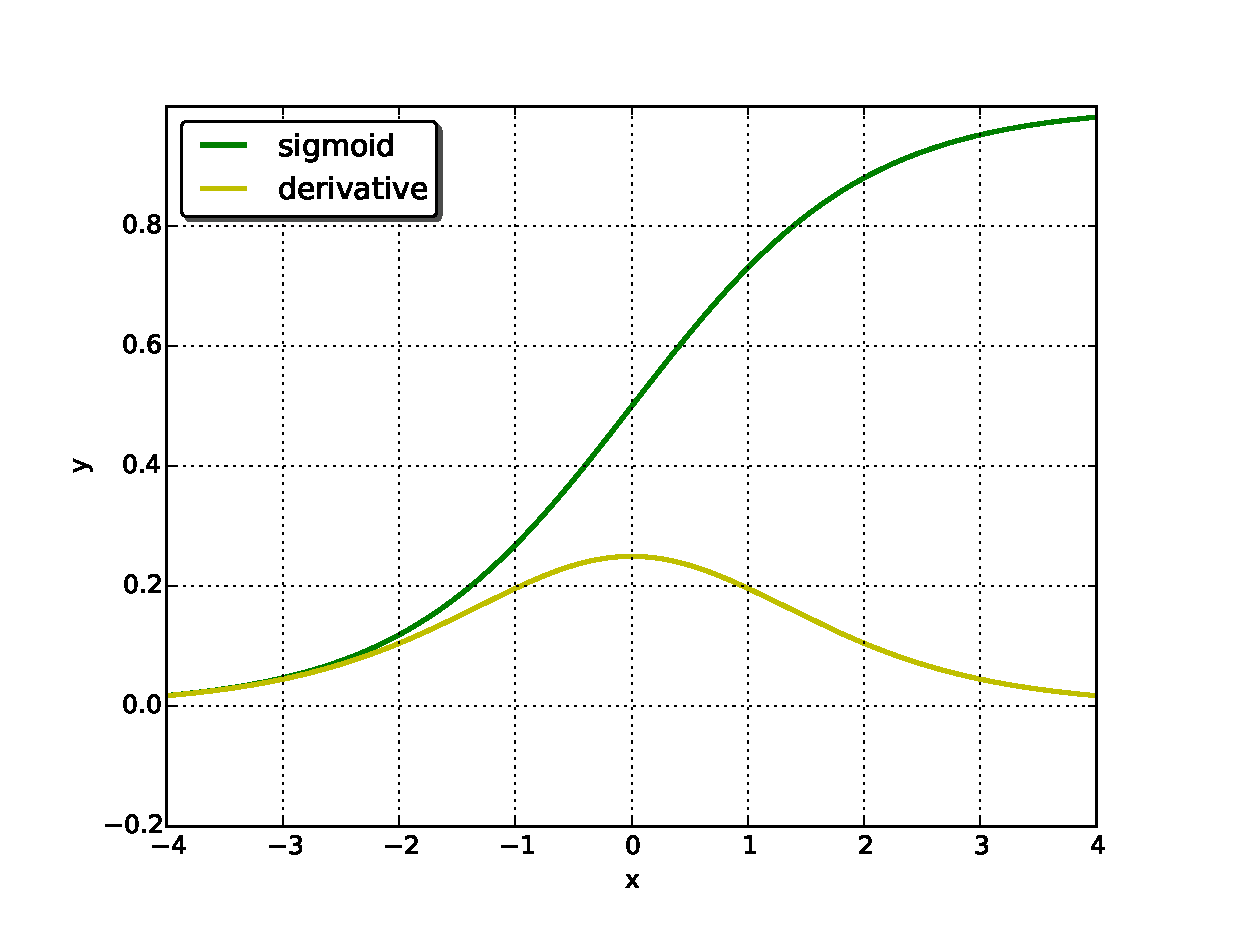
\includegraphics[width=0.9\textwidth]{sigmoid_and_deriv.eps}
  \caption{sigmoid and it's derivative}
\label{sigmoid_plot}
\end{figure}

\paragraph{Tanh}
\begin{align}
 tanh(x)&=\frac{e^x-e^{-x}}{e^x+e^{-x}} \\
 tanh'(x)&= 1 - tanh^2(x)  
\end{align}
As we can see from figure \ref{tanh_plot} tanh (and it's derivative) have a behaviour similar to the sigmoid one; Again we have two saturation region towards
infinity: that's typical of all squashing functions.



\begin{figure}[ht]
  \centering
    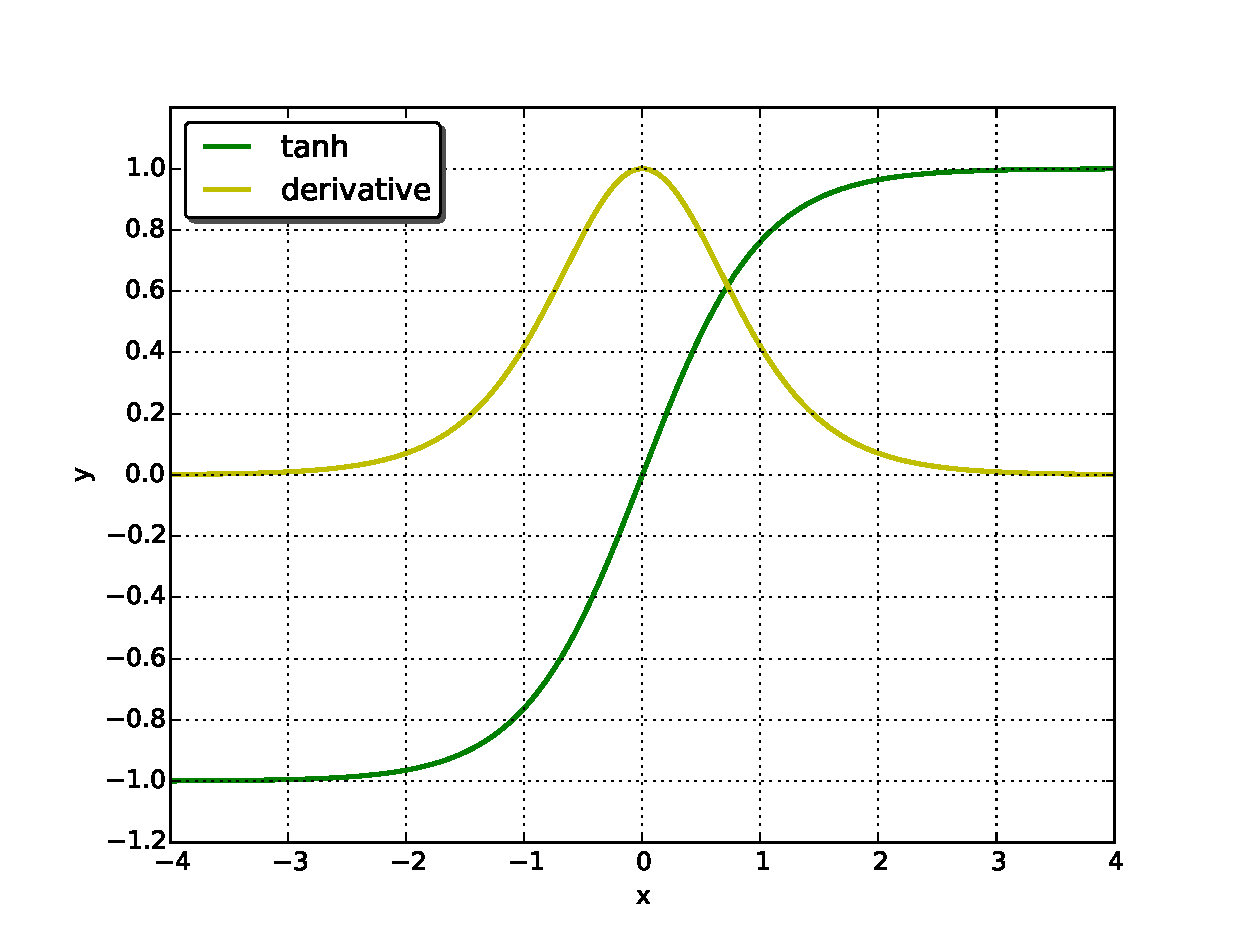
\includegraphics[width=0.9\textwidth]{tanh_and_deriv.eps}
  \caption{tanh and it's derivative}
\label{tanh_plot}
\end{figure}

\paragraph{ReLU}


\begin{align}
  ReLU(x)&=\begin{cases}
    x & \text{if $x>0$}.\\
    0 & \text{otherwise}.
  \end{cases} \\ 
   ReLU'(x)&=\begin{cases}
    1 & \text{if $x>0$}.\\
    0 & \text{otherwise}.
  \end{cases}
\end{align}
ReLU is a bit different from other activation function seen so far: the main difference is that's it's not a squashing function.
As we can see from figure \ref{relu_plot}, ReLU's derivative is the step function; it has only one \textit{saturation} region $(-\infty, 0]$ and a region in which is always takes value one, $(0,+\infty]$
This leads to the fact that we cannot learn to \textit{turn on} a switched off neuron ($x<0$), but we have no \textit{saturation} region toward infinity.

\begin{figure}[ht]
  \centering
    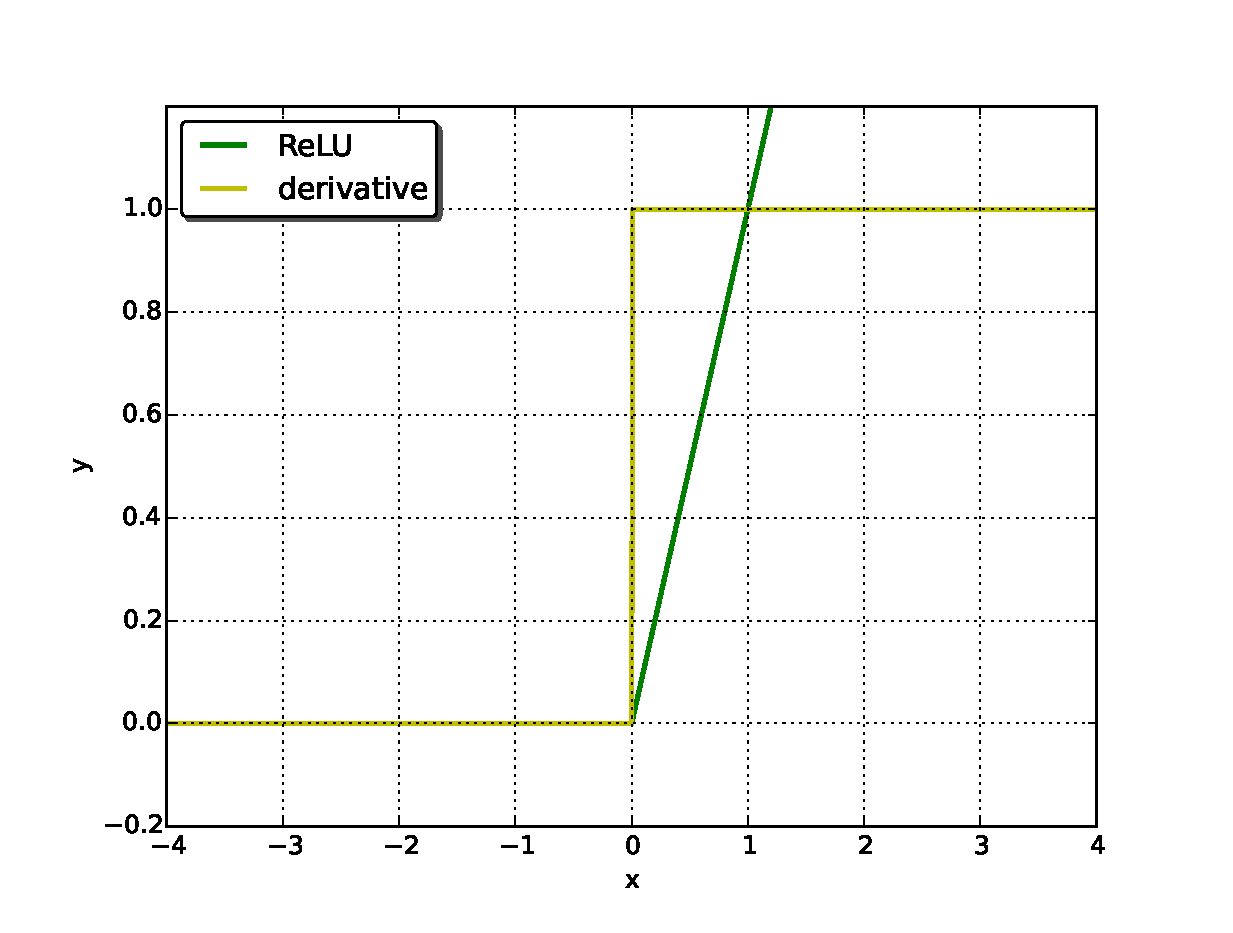
\includegraphics[width=0.9\textwidth]{relu_and_deriv.eps}
  \caption{ReLU and it's derivative}
\label{relu_plot}
\end{figure}

\section{On expressiveness}

\appendix
\chapter{Notation}

Let $F:\mathbb{R}^N \rightarrow \mathbb{R^M}$ be defined by
\begin{equation}
F(\vec{x}) = (f_1(\vec{x}),f_2(\vec{x}),\cdots,f_M(\vec{x}))) \text{    for some  } f_i:\mathbb{R}^N \rightarrow \mathbb{R}
\end{equation}

\begin{defn}[Derivative with respect to a vector]
 We define the derivative of $F(x(\vec{w}))$ with respect to a vector $\vec{w}$ of $p$ elements as the $M \times p$ matrix
\begin{equation}
\frac{\partial F}{\partial \vec{w}} \triangleq
\begin{bmatrix}
   \frac{\partial f_1}{\partial \vec{w}_1}    & \frac{\partial f_1}{\partial \vec{w}_2}                & \cdots      & \cdots       & \frac{\partial f_1}{\partial \vec{w}_p}  \\
   \frac{\partial f_2}{\partial \vec{w}_1}    & \frac{\partial f_2}{\partial \vec{w}_2}                & \cdots      & \cdots       & \frac{\partial f_2}{\partial \vec{w}_p}  \\
   \vdots                & \vdots           & \vdots      & \vdots       &\vdots\\
   \frac{\partial f_M}{\partial \vec{w}_1}    & \frac{\partial f_M}{\partial \vec{w}_2}                & \cdots      & \cdots       & \frac{\partial f_M}{\partial \vec{w}_p}
\end{bmatrix}
\end{equation}
\end{defn}


\begin{defn}[Derivative with respect to a matrix]
We define the derivative of $F(x(\mat{W}))$ with respect to a vector $\mat{W}$, being $W_j$ the $j^{th}$ column of a $p\times m$ matrix $W$ as the $M\times (p \cdot m )$ matrix:
\begin{equation}
\frac{\partial F}{\partial \mat{W}} \triangleq
\left[
\begin{array}{c|c|c|c}
\frac{\partial F}{W_1} & \frac{\partial F}{W_2} & \cdots & \frac{\partial F}{W_m} \\
\end{array}
\right]
\end{equation}
\end{defn}







\newpage
 \nocite{*}		 % Mostra in bibliografia anche gli oggetti non citati 
\bibliography{biblio}{}
\bibliographystyle{plain}


\end{document}     